% Created 2014-10-06 Mon 18:37
\documentclass[11pt,oneside]{memoir-article}
\usepackage{calculating-the-uposatha-moondays}
\renewcommand{\docVersion}{v0.1}
\renewcommand{\docUrl}{\href{https://github.com/profound-labs/calculating-the-uposatha-moondays/}{link}}
\hypersetup{ pdfauthor={Gambhiro Bhikkhu}, }
\author{Gambhiro Bhikkhu}
\date{\today}
\title{Calculating the Uposatha Moondays}
\hypersetup{
  pdfkeywords={},
  pdfsubject={},
  pdfcreator={Emacs 24.4.50.1 (Org mode 8.2.7c)}}
\begin{document}

\maketitle
\begin{tldr}
\begin{itemize}
\item The aim here is to describe the practical steps to calculate the
\emph{uposatha} Full- and New Moon days, and indicate the astronomical
cycles that underlie the method.
\item Alternate 30 and 29 day lunar months, 12 months make one year. Add
an extra month 7 times in every 19 years, add an extra day 11 times
in every 57 years.
\item Conventions on how to practise this can differ by countries and
groups, resulting in consistent but different calendars.
\item Unforseen adjustments to the predicted uposatha days in the
published Royal Calendar can be expected.
\end{itemize}
\end{tldr}

\begin{center}
\textbf{Unresolved Questions:}

\begin{itemize}
\item When is the adhikavara inserted?
\item Only Mahanikaya adds adhikavara?
\end{itemize}

This document is still work-in-progress and represents only what I've
been able to find description of. See the links in the \hyperref[sec-5]{Bibliography} or
download a zip of this document and sources.

Comments, corrections or further information would be greatly
appreciated. \texttt{\{\{\{email\}\}\}}
\end{center}

\chapter{Thailand, Mahānikāya Method}
\label{sec-1}
\section{Alternate 30 and 29 day months}
\label{sec-1-1}

Counting from the last Full Moon of the previous lunar year (which may
be in January), the first month is 30 days, the second is 29 days:

\begin{center}
\begin{tabular}{lll}
15 days & \GaNewmoon{} New Moon & First uposatha of the Cold Season\\
15 days & \GaFullmoon{} Full Moon & End of first month, 30 days\\
15 days & \GaNewmoon{} New Moon & \\
14 days & \GaFullmoon{} Full Moon & End of second month, 29 days\\
\end{tabular}
\end{center}

The \GaWaxingmoon{} Waxing- and \GaWaningmoon{} Waning Moons are on the 8th day.

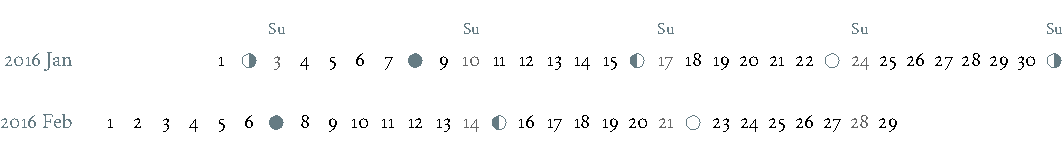
\includegraphics[width=\linewidth]{two-months.pdf}

Keep alternating 30 and 29 day months. One season is four months, one
year is three seasons: Cold-, Hot- and Rainy Season. In a year with
nothing special, the calendar is finished. See Table \ref{tbl-month-names}
for the Pali names of months and seasons.

In some years an extra month (adhikamāsa) or an extra day
(adhikavāra) has to be added.

\section{Adding the extra month}
\label{sec-1-2}

In Thai practice, the extra month (adhikamāsa) is a 30 day month
inserted after the 8th month (\emph{Āsāḷha}), at the end of the Hot
Season. The convention is to call this the 'second 8th' or 'second
\emph{Āsāḷha}', marked as 8/8.

Vassa starts after the 2nd Āsāḷha, on the day after the Full Moon
uposatha of 8/8.

\begin{center}
\begin{tabular}{llr}
order & name & days\\
\hline
\ldots{} &  & \\
8 & Āsāḷha & 29\\
8/8 & 2nd Āsāḷha & 30\\
9 & Savaṇa & 30\\
\end{tabular}
\end{center}

The extra month is added 7 times in every 19 year, in a repeating pattern of
3-3-2 - 3-3-3-2 years. See Table \ref{tbl-19yr-adhikamasa}.

\begin{table}[htb]
\caption{\label{tbl-19yr-adhikamasa}19-year cycles of the adhikamāsa\cite{hasapannyo-zodiac}}
\centering
\begin{tabular}{rrrr}
 & 1 & 1997 & 2016\\
 & 2 &  & \\
3 & 3 & 1999 & 2018\\
 & 4 &  & \\
 & 5 &  & \\
3 & 6 & 2002 & 2021\\
 & 7 &  & \\
2 & 8 & 2004 & 2023\\
 & 9 &  & \\
 & 10 &  & \\
3 & 11 & 2007 & 2026\\
 & 12 &  & \\
 & 13 &  & \\
3 & 14 & 2010 & 2029\\
 & 15 &  & \\
 & 16 &  & \\
3 & 17 & 2013 & 2032\\
 & 18 &  & \\
2 & 19 & 2015 & 2034\\
\end{tabular}
\end{table}

\section{Adding the extra day}
\label{sec-1-3}

The extra day (adhikavāra) is added 11 times in every 57 year.

\begin{quote}
It appears to be added every few years in the 3rd uposatha of the Hot Season
-- making it a fifteen-day uposatha instead of the expected
fourteen-day. King Mongkut apparently devised a method to abandon this
practice, but the issue remains a mistery\ldots{}\cite{hasapannyo-zodiac}
\end{quote}

\section{Major Moondays}
\label{sec-1-4}

Buddhist communities observe key annual events on the Full Moon
days of four lunar months, see Table \ref{tbl-major-moons}.

\begin{table}[htb]
\caption{\label{tbl-major-moons}Major Moondays}
\centering
\begin{tabular}{lll}
 & Lunar Month & \\
Māgha Pūjā & 3rd & \\
Visākha Pūjā & 6th & \\
Āsāḷha Pūjā & 8th & Entering Vassa on the next day\\
Assayuja Pūjā & 11th & Pavāraṇā Day, the end of Vassa\\
\end{tabular}
\end{table}

The Full Moon day is on the last day of a given month. The next month
starts on the following day (first day of the waning phase), thus the
first uposatha will be on a New Moon.

\chapter{Adding the extra month, Pali method}
\label{sec-2}

\emph{The following is adapted from Ajahn Khemanando for recent
years.}\cite{khemanando-adhikamasa}

Table \ref{tbl-cycle-adhikamasa} shows the 19-year cycle between
1997-2034.

\begin{table}[htb]
\caption{\label{tbl-cycle-adhikamasa}Adhikamāsa accoding to the Pali method}
\centering
\begin{tabular}{rrrrrlrr}
 &  &  &  & Month & Season & New & Full\\
\hline
 & 1 & 1997 & 2016 &  &  &  & \\
 & 2 &  &  &  &  &  & \\
3 & 3 & 1999 & 2018 & 5 & Hot & 4 & 8/8\\
 & 4 &  &  &  &  &  & \\
 & 5 &  &  & 2 & Cold & 12 & 5\\
3 & 6 & 2002 & 2021 &  & Cold & 12 & 5\\
 & 7 &  &  &  &  &  & \\
2 & 8 & 2004 & 2023 & 10 & Rainy & 8 & 12\\
 & 9 &  &  &  &  &  & \\
 & 10 &  &  &  &  &  & \\
3 & 11 & 2007 & 2026 & 7 & Hot & 4 & 8/8\\
 & 12 &  &  &  &  &  & \\
 & 13 &  &  & 3 & Cold & 12 & 5\\
3 & 14 & 2010 & 2029 &  & Cold & 12 & 5\\
 & 15 &  &  &  &  &  & \\
 & 16 &  &  & 12 & Cold & 12 & 5\\
3 & 17 & 2013 & 2032 &  & Cold & 12 & 5\\
 & 18 &  &  &  &  &  & \\
2 & 19 & 2015 & 2034 & 8 & Rainy & 8 & 12\\
\end{tabular}
\end{table}

\begin{description}
\item[{Month:}] the Thai lunar month into which the adhikamāsa is inserted
\item[{Season:}] the season in which the adhikamāsa fall in that
particular year
\item[{New and Full:}] the first and last uposatha of the 5-month season
in which the adhikamāsa falls, numbered in Thai
lunar months
\end{description}

If the adhikamāsa falls on the 2nd, 3rd, or 12th Thai lunar month,
there will be \emph{two} 8th months (8 and 8/8) the following year.

E.g. In 2001, the adhikamāsa comes as the 2nd lunar month in the
Cold Season, so the following year, 2002, has two 8th months (8 and
8/8). There will thus be \emph{ten} uposathas in the Cold Season, the
first being the New Moon of the 12th Thai lunar month (2001) and the
last being the Full Moon of the 5th Thai lunar month, 2002.
\chapter{Names of the months}
\label{sec-3}

Note on zodiacs, full moon at midnight, etc.

\begin{table}[htb]
\caption{Lunar and Solar Months and Zodiacs\cite{hasapannyo-zodiac}}\legend{\mA{} marks 29 day months having a 14 day New Moon (\emph{amāvasī cātuddasī}).}
\centering
\begin{tabular}{llll}
Season & Lunar Month & Solar Month & Solar Zodiac\\
 &  &  & (Western / Sanskrit)\\
\hline
Hemanta-utu & Magasira-māsa & December & Sagittarius / Dhanus\\
Cold Season & Phussa-māsa\mA & January & Capricorn / Makara\\
 & Māgha-māsa & February & Aquarius / Kumbha\\
 & Phagguṇa-māsa\mA & March & Pisces / Mīna\\
\hline
Gimha-utu & Citta-māsa & April & Aries / Meṣa\\
Hot Season & Visākha-māsa\mA & May & Taurus / Vṛṣabha\\
 & Jeṭṭha-māsa & June & Gemini / Mithuna\\
 & Āsāḷha-māsa\mA & July & Cancer / Karkaṭa\\
\hline
Vassāna-utu & Savaṇa-māsa & August & Leo / Siṃha\\
Rainy Season & Bhaddapāda-māsa\mA & September & Virgo / Kanyā\\
 & Assayuja-māsa & October & Libra / Tulā\\
 & Kattika-māsa\mA & November & Scorpio / Vṛścika\\
\end{tabular}
\end{table}
\chapter{The Thai luni-solar calendar}
\label{sec-4}

Luni-solar calendars are constructed so to count years according to
the \emph{solar} cycle, but to count months according to the \emph{lunar} cycle.

\begin{center}
\begin{tabular}{ll}
tropical year\footnotemark of the Earth & 365.24219 days\\
synodic month\footnotemark of the Moon & \textasciitilde{}29.53 days, can vary up to 7 hours\\
\end{tabular}
\end{center}\footnotetext[1]{tropical year: the time it takes the Earth to
complete an orbit around the Sun}\footnotetext[2]{synodic month: the time it takes the Moon to reach
the same visual phase

The epoch of the Thai calendar is 25 March 638 CE.

The Thai luni-solar calendar is \emph{procedural}, it uses a couple of
constant, key numbers derived from astronomical observations, and
applies a series of mechanical calculations (i.e. the "rules") again
and again to generate the dates of lunar phases and new years.

\begin{quote}
This working is deliberately concise, since it thereby reflects how
the calculation would have been made by a South East Asian calendrist.
Each stage is subjected to an operation learnt by rote, and the
underlying theory disappears from view. The rote operations, however,
will provide a valid answer for any date in any year. It seemed
greatly preferable to set out the procedure thus starkly, rather than
to give a detailed exposition of what is involved.\cite{eade-interpolation}
\end{quote}

Southeast Asian astronomers refined a fraction to obtain the length of
the year:

\begin{equation}
\frac{292207}{800} = 365.25875 \text{days}
\end{equation}\cite{eade-interpolation}

This is 0.01656 days longer than the modern measurement (1 day in \textasciitilde{}60
years). Remarkably, the \emph{suriyayatra} accounts for this and generates
accurate results:

\begin{quote}
For instance, a Pagan inscription of 14 April 1288 AD maintains that
at midnight the sun's position was 0 signs, 19 degrees and 59 minutes:
the computer program returns 0 19 59.\cite{eade-calendrical}
\end{quote}

Nonetheless, the calendar dates published in Thailand in a given year
reflect not only these principles, but also additional adjustments
which cannot be forseen or retraced.

\begin{quote}
The historical record however, frequently defies prediction, forcing
the conclusion that the pressure upon the \emph{horas} (astronomers /
astrologers) was not to follow the "rules" but merely, within some
more leisurely constraints, to ensure that the calendar did not get
out of control.\cite{eade-calendrical}
\end{quote}}

\section{Year Types}
\label{sec-4-1}

We are concerned with three types of calendar years:

\begin{description}
\item[{Cal A}] Normal with 354 days
\item[{Cal B}] Adhikavāra with 355 days
\item[{Cal C}] Adhikamāsa with 384 days
\end{description}

Comparing these to normal and solar leap years:

\begin{center}
\begin{tabular}{lrrr}
 & A & B & C\\
Lunar & 354 & 355 & 384\\
Solar & 365 & 365 & 365\\
difference & $\backslash$+11 & $\backslash$+10 & -19\\
\hline
 & A & B & C\\
Lunar & 354 & 355 & 384\\
Solar Leap & 366 & 366 & 366\\
difference & $\backslash$+12 & $\backslash$+11 & -18\\
\end{tabular}
\end{center}

\section{Adhikamat years}
\label{sec-4-2}

The \emph{suriyayatra} principle to determine adhikamat years is:

\begin{quote}
"If the day of \emph{thaloengsok} (astronomical New Year)
lies either within 25 to 29 (in Citta-māsa) or 1 to 5 (in
Visākha-māsa), then the year is adhikamat."\cite{prasert-ngan}
\end{quote}

The \emph{thaloengsok} is the value of T in Figure \ref{fig-suriyayatra}.

\section{Adhikawan years}
\label{sec-4-3}

\begin{quote}
Two components of the \emph{suriyayatra} are known as the \emph{kammacubala} and
the \emph{avoman}, and it is the values of these two elemets at the start
of the year that determine the matter:

\begin{itemize}
\item if the kammacubala value is 207 or less, then the year is leap year
\item in a leap year, if the avoman is 126 or less, the year will have an
extra day
\item in a normal year, if the avoman is 137 or less, the year will have
and extra day\cite{eade-interpolation}
\end{itemize}
\end{quote}

The \emph{kammacubala} and \emph{avoman} are the value of K and A in Figure
\ref{fig-suriyayatra}.

In Thailand, years with an extra month are not allowed to also have an
extra day, and the adhikawan will be assigned to the next year.

\section{Suriyayatra formulas}
\label{sec-4-4}

\begin{figure}[h]
\caption{Finding astronomical values with the /suriyayatra/ calculation\cite{eade-interpolation}}
\legend{Start with Y, the given Common Era year. Significant values are assigned names. K for \emph{kammacubala}, A for \emph{avoman}, N for \emph{thaloengsok} (the New Year).}
\label{fig-suriyayatra}
\begin{eqnarray*}
a & = & ((Y - 638) * 292207) + 373 \\
h & = & \lfloor a/800 + 1 \rfloor \\
K & = & 800 - a \bmod 800 \\
A & = & ((h*11) + 650) \bmod 692 \\
b & = & \lfloor ((h*11) + 650) / 692 \rfloor \\
T & = & (b + h) \bmod 30
\end{eqnarray*}
\end{figure}

\begin{center}
\begin{tabular}{rrrrrlrr}
 &  &  &  & year & type & Asalha & 2nd Asalha\\
\hline
 &  & 0 &  & 1320 & m & 19:42 & 22:24\\
0 &  & 1 &  & 1321 & d & 21:05 & \\
1 &  & 2 &  & 1322 &  & 20:40 & \\
2 &  & 3 & 3 & 1323 & m & 19:12 & 22:00\\
3 &  & 4 &  & 1324 &  & 20:38 & \\
4 & 4 & 5 &  & 1325 & d & 19:34 & \\
5 &  & 6 & 3 & 1326 & m & 19:38 & 22:05\\
6 &  & 7 &  & 1327 &  & 21:15 & \\
7 &  & 8 & 2 & 1328 & m & 19:20 & 22:55\\
8 &  & 9 &  & 1329 &  & 21:48 & \\
9 & 5 & 10 &  & 1330 & d & 20:26 & \\
10 &  & 11 & 3 & 1331 & m & 19:59 & 22:50\\
11 &  & 12 &  & 1332 &  & 21:20 & \\
12 &  & 13 &  & 1333 &  & 20:02 & \\
13 &  & 14 & 3 & 1334 & m & 19:03 & 21:33\\
14 & 5 & 15 &  & 1335 & d & 20:40 & \\
15 &  & 16 &  & 1336 &  & 20:44 & \\
16 &  & 17 & 3 & 1337 & m & 19:44 & 22:19\\
17 &  & 18 &  & 1338 &  & 21:11 & \\
18 &  & 19 & 2 & 1339 & m & 19:45 & 22:35\\
19 & 5 &  &  & 1340 & d & 21:05 & \\
 &  &  &  &  &  &  & \\
 &  &  &  &  &  &  & \\
 &  &  &  &  &  &  & \\
\end{tabular}
\end{center}
\chapter{Bibliography}
\label{sec-5}


\bibliographystyle{plain}
\bibliography{bibentries}

\chapter{Colophon}
\label{sec-6}

Written in Org-mode. Sources are at \texttt{Github}.

Comments, corrections or further information would be greatly
appreciated.

\texttt{Gambhiro Bhikkhu <gambhiro.bhikkhu.85@gmail.com>}

Last updated: 
% Emacs 24.4.50.1 (Org mode 8.2.7c)
\end{document}
